\documentclass[12pt,a4,notitlepage]{report}

\usepackage{verbatim,graphicx,fancyvrb}

% \input{epsf}            % to allow postscript inclusions

\raggedbottom             % try to avoid widows and orphans
\sloppy
% \clubpenalty1000%
% \widowpenalty1000%

\setlength{\parindent}{0cm}
\setlength{\parskip}{2ex plus 1ex minus 0.5ex}
\addtolength{\evensidemargin}{-1.5cm}
\addtolength{\oddsidemargin}{-1.5cm}
\addtolength{\textwidth}{2.6cm}
\addtolength{\topmargin}{0.5cm}
\addtolength{\textheight}{2cm}
\addtolength{\footskip}{0.5cm}

\renewcommand{\textfraction}{0.15}
\renewcommand{\topfraction}{0.85}
\renewcommand{\bottomfraction}{0.65}
\renewcommand{\floatpagefraction}{0.60}

\renewcommand{\_}{\texttt{\symbol{95}}}
\newcommand{\<}{\texttt{\symbol{60}}}
\renewcommand{\>}{\texttt{\symbol{62}}}
\newcommand{\class}[1]{\textbf{#1}}
\newcommand{\scopendpoint}[1]{\texttt{#1}}
\newcommand{\variable}[1]{\texttt{#1}}
\newenvironment{pseudocode}{\begin{slshape}\begin{tabbing}\hspace*{0.5cm}\=\hspace*{0.5cm}\=\hspace*{0.5cm}\= \kill }{\end{tabbing}\end{slshape}}
\DefineVerbatimEnvironment{code}{Verbatim}{}
\newcommand{\implies}{\Rightarrow}

\includeonly{propbody}

%\renewcommand{\baselinestretch}{1.1}    % adjust line spacing to make
%                                        % more readable

\begin{document}

\bibliographystyle{plain}

%%%%%%%%%%%%%%%%%%%%%%%%%%%%%%%%%%%%%%%%%%%%%%%%%%%%%%%%%%%%%%%%%%%%%%%%
% Title

\pagestyle{empty}

\hfill{\LARGE \bf Cheryl Hung}

\vspace*{30mm}
\begin{center}
\Huge
{\bf Gesture-controlled Robotics \\
using the Vicon Motion Capture System} \\
\vspace*{25mm}
Computer Science Tripos \\
\vspace*{5mm}
King's College \\
\vspace*{5mm}
\today  % today's date
\end{center}

\cleardoublepage

%%%%%%%%%%%%%%%%%%%%%%%%%%%%%%%%%%%%%%%%%%%%%%%%%%%%%%%%%%%%%%%%%%%%%%%%%%%%%%
% Proforma, table of contents and list of figures

\setcounter{page}{1}
\pagenumbering{roman}
\pagestyle{plain}

\chapter*{Proforma}

{\large
\begin{tabular}{ll}
Name:               & \bf Cheryl Hung                       \\
College:            & \bf King's College                     \\
Project Title:      & \bf Gesture-controlled Robotics using the \\
                    & \bf Vicon motion capture system \\
Examination:        & \bf Computer Science Tripos, 2009        \\
Word Count:         & \bf wordcount \\
Project Originator: & Cheryl Hung                    \\
Supervisor:         & Cecily Morrison, Laurel Riek                    \\ 
\end{tabular}
}

\section*{Original Aims of the Project}

The original 

To write a gesture recognition system which converts a stream of coordinates into commands to drive a robot.

\section*{Work Completed}

Preprocessing
Recognition methods: Heuristic, Neural, Markov, Hybrid
Robot control
Full simulations of coordinates and control

\section*{Special Difficulties}

None
 
\newpage
\section*{Declaration}

I, Cheryl Hung of King's College, being a candidate for Part II of the Computer Science Tripos, hereby declare that this dissertation and the work described in it are my own work, unaided except as may be specified below, and that the dissertation does not contain material that has already been used to any substantial extent for a comparable purpose.

\bigskip
\leftline{Signed }

\medskip
\leftline{Date }

\cleardoublepage

\tableofcontents

\listoffigures

\newpage
\section*{Acknowledgements}

Acknowledgements

%%%%%%%%%%%%%%%%%%%%%%%%%%%%%%%%%%%%%%%%%%%%%%%%%%%%%%%%%%%%%%%%%%%%%%%
% now for the chapters

\cleardoublepage        % just to make sure before the page numbering
                        % is changed

\setcounter{page}{1}
\pagenumbering{arabic}
\pagestyle{headings}

\chapter{Introduction}

New paradigms for human-computer interaction are becoming a reality. Amongst consumer goods, new ways of interaction are forcing a rethink beyond the keyboard and mouse. The Apple iPhone is the first touchscreen cellular phone to be widely adopted, while the Nintendo Wii brings accelerometer based control to home gaming. The Opera browser uses mouse gestures for navigational input, while the Microsoft Surface is aimed towards diverse markets such as corporate events and restaurants.

The philosophy which is common to these systems is defined by the term ``ubiquitous computing''. The aim is to allow intuitive, natural interaction so that anybody (in theory) can use them without training, but instead by mirroring or mimicking behaviour of the real world.

Conversely, robots have generally been operated by skilled engineers and researchers. The motivation was to bring the power of human intuition, using techniques from machine learning, to the human-machine interface. The medium that I chose to investigate and exploit is gesture recognition, a specialization of pattern recognition.

While machine vision is one option for solving this problem, motion capture systems provide far more detailed location data, down to hundredths of a millimeter. Rather than allowing users full freedom of gestures, I chose to train on a finite set of predefined gestures, converting these into commands that are used to drive the robot. 

The two computational models used internally for this translation are Artificial Neural Networks and Hidden Markov Models. Gesture recognition is really a two-phase problem; the training with prerecorded datasets and the run-time interpretation. 

This project uses machine learning techniques for gesture recognition in order to control a remote vehicular robot. Three very different approaches were taken to the same problem; a heuristic evaluator, Artifical Neural Networks, and Hidden Markov Models. The gesture data was recorded from a motion capture system using arm and body markers for training purposes and was preprocessed for invariance to translation and rotation before feature extraction. A voting system was implemented to aggregate the results and intepret the real time data as commands. Furthermore, an extension for multiple users was implemented, and the system demonstrated successfully on live motion capture data to control physical hardware.

\chapter{Preparation}

\section{Requirements Analysis}

The project is divided into three phases; preprocessing of motion capture data, recognition and intepretation into commands, and execution on hardware. 

\section{Hardware}

The main requirements of the hardware were:

\begin{enumerate}
\item It should  have a range of commands it is willing to accept, in order to allow training of multiple gestures. A simple vehicle sufficed for this purpose.
\item It should have wireless capabilities for independant movement, and sensors and webcam for the collision based game.
\item A high level API or library is preferred, for ease of development.
\item Commercially available robots makes purchasing for multiuser applications easier.
\item High battery life and low power consumption, for testing purposes.
\item Low cost (see budgeting for more)
\end{enumerate}

The main alternatives considered were:
\begin{enumerate}
\item Lego Mindstorms, already owned by the Computer Laboratory and including a C++ API, with purchased modules for wireless and touch sensors. This was dismissed as building a vehicle and testing for range of movement etc. would take excessive development time.
\item iRobot Roomba, a low cost vacuum cleaning robot with bump sensors, with third party peripherals for wireless and webcam. Reaching the serial ports on the Roomba would require removal of hardware and deconstruction of the vacuum innards.
\item iRobot Create, an educational robot similar to the Roomba, without vacuum parts. A device for wireless could be attached by serial cable. A setup based on the OLPC Telepresence {reference: OLPC Telepresence} also provided a Python library for interfacing with both the laptop's webcam and robot's motors and bump sensors.
\end{enumerate}
{Command module?}

{diagram: robot}

The budget was \pounds 500, funded equally by the Computer Laboratory Outreach programme and King's College. The final expenditure came to \pounds 585 as follows:

Two iRobot Creates at \$229.99 = \pounds 306.80
OLPC XO laptop @ \$220.00 = \pounds 151.86
OLPC XO laptop @ \$170.00 = \pounds 117.35
UK/US Step Down Adapter = \pounds 8.99

Total: \pounds 585.00

The main reason for the increase was that the basic iRobot Create comes without a rechargeable battery, and requires 12 AA batteries per robot per hour. The upgraded package comes with a command module as well as rechargeable battery; however it was found that the command module cannot be used, as it considers the laptop attached via USB to be a peripheral rather than the laptop being the USB master device to the robot slave.

\section{Motion Capture System}

The Vicon Motion Capture system in the Rainbow Group is controlled by Tarsus. This software collates the data from the ten infra-red cameras to reconstruct the three dimensional marker positions in real time, and further combines these into either user-defined objects or full skeletons. There were two choices to be considered; the objects (body parts), and the gestures to be recognised.

The objects needed firstly for input to a gesture, and secondly representing the user's position so that gestures can be calculated invariant to translation, rotation and spatial displacement. For the gesture input, one or two hands or arms were considered; two gives a wider range of movement (and thus a larger input space) and forearms have more rigidity than hands, giving better recognition rates from the Vicon system. Options for positional data were belt, hat and body. The belt was easily occluded and confused by the arm markers, while the hat gave poor rotational data due to the independent movement of the head. The final configuration chosen was twelve markers spread across two arms and body (upper chest and back).

{diagram: markers}

The data outputted is six data values per object; an Axis Angle triplet for rotation and a triplet for global translation in mm. An alternative rotation system which is also available is Euler angles.

In order to simplify data processing while providing adequate control over the robot, most of the pre-set gestures were constrained to one arm movement within two dimensions (x-z or y-z planes in a z-up world). The commands chosen to provide basic steering and speed were accelerate, decelerate, turn left, turn right and start/stop, the last being a test case for a more complex gesture, in this case a single clap at chest level. Figure \ref{gestures} shows the arm gestures for each command.

\begin{figure}
\centering
\includegraphics[scale=0.3,angle=0]{images/accel.ps}
\includegraphics[scale=0.3,angle=0]{images/decel.ps}
\includegraphics[scale=0.3,angle=0]{images/left.ps}
\includegraphics[scale=0.3,angle=0]{images/right.ps}
\includegraphics[scale=0.3,angle=0]{images/startstop.ps}
\caption{Left to right: arm gestures for \textit{accelerate}, \textit{decelerate}, \textit{turn left}, \textit{turn right}, and \textit{start/stop}.}
\label{gestures}
\end{figure}

\subsection{Axis Angles}

Axis angles are also known as exponential coordinates or rotation vectors. This parametrizes orientation by a three dimensional Cartesian vector, describing a directed axis and the magnitude of rotation. The following rotation matrix is used to rotate around an arbitrary axis where (x,y,z) is a unit vector on the axis of rotation, and theta is the angle of rotation.

{reference: Graphics Gems}

$(x,y,z)$\\

$\theta = \sqrt{x^2 + y^2 + z^2}$\\

$c = \cos(\theta)$\\
$s = \sin(\theta)$\\
$t = 1-c $\\

$R =
\left( \begin{array}{ccc}
      tx^2+c & txy+sz & txz-sy\\
		txy-sz & ty^2+c & tyz+sx\\
		txz+sy & tyz-sx & tz^2+c\\
\end{array} \right)$

\subsection{Euler Angles}

With Euler angles, the rotation matrix is decomposed into three rotations from a reference frame, $(x,y,z)$. The rotated orientation system is denoted in upper case letters, (X,Y,Z). The line of nodes (N) is the line of intersection between the xy and XY coordinate planes, and the new coordinate system is parametrized by $(\alpha,\beta,\gamma)$.

In the z-x-z convention,

\begin{itemize}
\item $\alpha$ is the angle between the x-axis and the line of nodes, modulo $2\pi$
\item $\beta$ is the angle between the z-axis and the Z-axis, modulo $\pi$
\item $\gamma$ is the angle between the line of nodes and the X-axis, modulo $2\pi$
\end{itemize}

\begin{figure}[hb]
\centering
\includegraphics[scale=0.2,angle=0]{diagrams/eulerangles.ps}
\caption{Euler Angles}
\label{eulerangles}
\end{figure}

However, when the $xy$ and $XY$ planes are identical and the $z$ and $Z$ axes are parallel, the Euler system is subject to a phenomenon known as gimbal lock, since not all points in the coordinate system can be uniquely identified. Euler angles are also prone to angle flips at the extremities of the ranges of $\alpha,\beta,\gamma$. For this reason, Euler angles are harder to deal with than axis angles, which vary smoothly.

\section{Pattern recognition}

There are many different techniques used for pattern recognition. The purpose of the pattern recognition phase is to classify the observations into categories, based on extracted features. For supervised learning, a training set of patterns is labelled with the correct classification; unsupervised learning (such as the K-means clustering algorithm) evaluate the raw, unlabelled data and attempt to infer the patterns, for example by minimizing the root mean squared error based on Euclidean distance. However given the set of gestures are fixed for this application, the algorithms for supervised learning have higher accuracy ratings so unsupervised learning will not be considered further.

Statistical techniques for pattern recognition are based on finding a classifier
$ h: X \mapsto Y $ which maps $x \in X$ to $y \in Y$ in a close approximation to the actual ground function $ g: X \mapsto Y $ where the training set $ (\mathbf x_1,y_1), ... , (\mathbf x_n, y_n) $ are instances of $X \times Y$ (the Cartesian product of the $X$ and $Y$ domains).

Among the more popular techniques are Support Vector Machines, naive Bayes classifier, k-nearest neighbour, neural networks and Hidden Markov Models. I chose the latter two as an example of a general classifier and temporal classifier respectively.

\subsection{Neural Networks}

An artificial neural network is an interconnected set of nodes which individually perform simple processing, but exhibits complex behaviour as a whole system. This is the connectionist approach to pattern recognition from large sets of data, inspired by  biological neural networks. Each unit combines the inputs by means of an activation function, which fires non-linearly given sufficient input. Common choices for the activation function are the tanh function or the sigmoid function, which have the property of being differentiable:

\[ \phi(v_i) = 1/(1+e^{-v_i}) \]

{diagram: single neuron}

$w_{ji}$ connects node $i$ to node $j$ \\
$a_{ij}$ is the activation for node, the weighted sum of the inputs = $\sum_i {w_{ji}z_i}$ \\
$g$ is the activation function \\
$z_j = g(a_j)$ \\
bias input = 1

The most common model is the multilayer perceptron, where the overall structure is feedforward and there are three layers of nodes; an input layer, a hidden layer and an output layer. 

{diagram: multilayer perceptron}

Since this is a supervised learning technique, the first phase is to present training data. The goal is to adjust the weights $w$ so as to minimise the overall error, denoted ${E}(\mathbf w)$. The training sequence is a vector of labelled inputs:

\[ s = ((\mathbf x_1,y_1), ... , (\mathbf x_m, y_m)) \]

The backpropagation algorithm is an application of gradient descent for minimization of error. The first stage is to initialize w to a random set of weights. Calculate $E (\mathbf w)$; if this is greater than a threshold value, calculate the gradient $\partial E (\mathbf w) / \partial \mathbf w $ of $E(\mathbf w )$ at each point wi and adjust the weight vector to lower the error:

\[
\mathbf w_{i+1} = \mathbf w_i - \alpha \left. \frac {\partial E(\mathbf w)} {\partial \mathbf w} \right| \mathbf w_i
\]

The forward propagation stage is to calculate $a_j$ and $z_j$ for all nodes, given an input example $p$.

\[
\frac {\partial E_p(\mathbf w)} {\partial w_{ji}} = \frac {\partial E_p(\mathbf w)} {\partial a_j} \frac {\partial a_j} {\partial w_{ji}} = \delta_j z_i
\]

where $\delta j = \frac {\partial E_p\mathbf w} {\partial a_j}$
and $ \frac {\partial a_j} {\partial w_{ji}} = \frac {\partial} {\partial w_{ij}} \left( \sum_k {z_kw_{jk}} \right) = z_i$

There are two cases for calculating $\partial_j$:

1. $j$ is an output node

\[
\delta j = \frac {\partial E_p (\mathbf w)} {\partial a_j} \\
 = \frac {\partial E_p (\mathbf w)} {\partial z_j} \frac {\partial z_j} {\partial a_j} \\
 = \frac {\partial E_p (\mathbf w)} {\partial z_j}  g'(a_j)
\]

2. $j$ is not an output node

\[
\delta j = \frac {\partial E_p (\mathbf w)} {\partial a_j}
 = \sum_{k \in \{k_1, k_2,\ldots,k_q\}} \frac {\partial E_p (\mathbf w)} {\partial a_k} \frac {\partial a_k} {\partial a_j}
 = g'(a_j) \sum_{k \in \{k_1, k_2,\ldots,k_q\}} {\delta_k w_{kj}}
\]

since $ \frac {\partial a_k} {\partial a_j} = \frac {\partial} {\partial a_j} \left( \sum_{k \in \{k_1, k_2,\ldots,k_q\}} { w_{ki} g(a_i) } \right) = w_{kj} g'(a_j) $

This gives the \textit{back-propagation formula}\cite{NeuralPat}:
\[
\delta j = g'(a_j) \sum_{k \in \{k_1, k_2,\ldots,k_q\}} {\delta_k w_{kj}}
\]

The importance of this result is the resulting reduction in time complexity, as training neural networks is very time consuming. The majority of the work is done calculating $a_{ij} = \sum_i {w_{ji}z_i}$. There are $W$ derivatives to calculate for $W$, letting $W$ be the total number of weights and biases. The naive approach of explicit evaluating each derivative in $O(W)$ operations is therefore $O(W^2)$ in time complexity. By contrast,  backpropagation (using $\frac {\partial E_p(\mathbf w)} {\partial w_{ji}} = \delta_j z_i$ to calculate the derivatives) reduces the computational complexity to $O(W)$.

\subsection{Hidden Markov Models}

First order Markov processes are a class of statistical model which state that the probability of being in some future state is only dependant on the current state, also known as the memoryless model since the ``memory" or past states have no effect on the next state.

\[ Pr(S_t|S_{0:t-1}) = Pr(S_t|S_{t-1}) \]

where $S_{0:t-1} = (S_0,S_1,...S_{t-1})$


{diagram: hidden markov models}

At each time $t$, a symbol is emitted from state $i$. For a Bakis HMM, at $t+1$ the only options are to stay in state $i$ or move to state $i+1$. Each state is parametrized by an emission probability of staying in the same state and a transition probability of moving to state $i+1$.

A Hidden Markov Model is one where these probabilities characterizing the states are unknown, and for a training sequence, it is unknown which state the observation lies in. To find the probabilities, the Baulm-Welch algorithm takes a vector of training sequences and iterates using Expectation-Maximization. The expectation is calculated by the forward-backward algorithm, which is an example of dynamic programming - the use of memoization to save recomputing solutions to sub-problems.

For a Markov Model, $Pr(E_t|S_t)$ is the sensor model and $Pr(S_t|S_{t-1})$ is the transition model. $Pr(S_0)$ denotes the prior state.\cite{AIModern} The assumption is that the probabilities do not change over time, as the observations are stationary processes.

The forward-backward algorithm solves the task of smoothing; deducing the previous states from the current state, $Pr(S_t|e_{1:t})$ for $0 \leq T < t$. 

{latex:

The forward pass calculates $f_{1:t} = Pr(S_t|e_{1:t})$, passing $f_{1:t}$ as a forward message:
\begin{eqnarray*}
Pr(S_T | e_{1:t}) &=& Pr(S_T | e_{1:T}, e_{T+1:t}) \\
&=& c Pr(S_T | e_{1:T}) Pr(e_{T+1:t} | S_T,e_{1:T}) \\
&=& c Pr(S_T | e_{1:T}) Pr(e_{T+1:t} | S_T) \\
&=& c f_{1:T} b_{T+1:t} \\
\end{eqnarray*}
			
where $b_{T+1:t} = Pr(e_{T+1:t}|S_T)$ is the backward message for computing backwards probabilities:

\begin{eqnarray*}
\mbox{Initialisation: }b_{t+1:t} &=& Pr(e_{t+1:t}|S_t) = (1,...1) \\
b_{T+1:t} 	= Pr(e_{T+1:t}|S_T) &=&  \sum_{s_{T+1}} Pr(e_{T+1:t}, s_{T+1} | S_T) \\
						&=& \sum_{s_{T+1}} Pr(e_{T+1:t} | s_{T+1}) Pr(S_{T+1} | S_T) \\
						&=& \sum_{s_{T+1}} Pr(e_{T+1:t}, e_{T+2:t} | s_{T+1}) \\
						&=& \sum_{s_{T+1}} Pr(e_{T+1} | s_{T+1}) Pr(e_{T+2:t} | s_{T+1}) Pr(s_{T+1}|S_T) \\
						&=& \sum_{s_{T+1}} * Sensor model * b_{T+2:t} * Transition model \\
						&=& BACKWARDS(e_{T+1:t}, b_{T+2:t}) \\
\end{eqnarray*}

This smooths all points $1:t$ in time $O(t^2)$. By storing the computed results for $f_{1:T}$ and using these in the computation of $b_{T+1:t}$, this is reduced to $O(t)$.

Matrix multiplication to calculate f
Re-estimation

\section{Feature extraction}

Neural networks have a fixed number of input nodes and so variable length data must be converted to a fixed size feature vector. This technique, known as dimension reduction, also reduces the search space significantly, which reduces training times and can improve recognition rates.

There are several ways of doing this. For a discretely sampled time series, as the position data, the Discrete Fourier Transform encodes the signal as a coefficients of linear combinations of basis functions in a new frequency domain. Haar wavelets are an alternative method which also uses linear combinations of wavelet functions, which can represent discontinuities better than the Fourier method.

However these techniques were deemed excessively complex for the purposes of gesture recognition with a finite set of planar gestures. The simpler method of extracting axis-aligned ranges is sufficient for distinguishing the gestures without adding the computational overhead of these other techniques.

\section{Tools}

Subversion was used for version control, together with Google Code Project Hosting. The libraries used were:

Joone: Java Object Oriented Neural Engine \\
Jahmm: Java Hidden Markov Model \\
SCOP: Server COmmunication Protocol \\
PyRobot: robot and laptop control, motors, sensors and webcam \\
Tarsus: motion capture and object reconstruction \\

The majority of the system was developed under Ubuntu Linux, using NEdit and GEdit. The XO laptops run a modified version of Fedora Linux, while the PC used during live capture runs Windows XP.

This dissertation was typeset using \LaTeX.

\section{Languages}

The choice of languages was based on ease of development, portability, availability of libraries, and type safety. Python was chosen for readability and rapid prototyping, while Java was used for interfacing with powerful libraries. In a few cases certain classes have been prototyped in Python before being ported to Java.

The robot control library, PyRobot, is written in Python. Cecily Morrison's client and both pattern recognition engines are Java. Message passing of simple string data is handled by SCOP, which has ports to both Python and Java.

Since the OLPC XO runs a modified version of Fedora Linux, the Tarsus system runs on Windows XP and the development environment was Ubuntu Linux, using architecture independent languages makes it easy to perform processing on a more powerful computer to the XO laptop.

\chapter{Implementation}

\section{System Overview}

\begin{figure}
\centering
\includegraphics[scale=0.6,angle=0]{diagrams/systemdiagram.ps}
\caption{System Diagram}
\label{sysdiag}
\end{figure}

Figure \ref{sysdiag} shows how components are decoupled for re-usability. During training, the training sequences are read from disk and preprocessed to form data for training the pattern recognition modules. When live, the data capture subsystem sends double arrays of raw data values to the SCOP server. The preprocessing module additionally listens to the event stream for gesture data. The output from all three services is interpreted as one of five commands by Control and is sent to the SCOP server on a different stream. For testing purposes, a GUI provides alternative input methods of mouse and keystrokes.

The relay program on the XO laptop converts this into drive commands and the PyRobot library handles low level opcodes. The monitor shows the output for a turtle program which responds to the same commands, again for test purposes.

Message passing provides inter-language communication via an SCOP server running on the SRCF.

\subsection{Component Interfaces}

All SCOP messages are ASCII string messages. Each class that interacts with the server has a name and can express an interest in one or more streams, or endpoints by opening sockets.

NB: All names containing \verb^p1^ have \verb^p2^ equivalents.

\subsection{Protocols and data formats}

\begin{tabular}{l|p{2.5cm}p{4.5cm}p{4.5cm}}
\rule[-2mm]{0mm}{3mm} & Endpoint & Event sources & Event sinks\\
\hline
\rule{0mm}{4.5mm}\variable{coordsserver} & \scopendpoint{p1coords} &
\scopendpoint{capturep1}, \scopendpoint{simulatep1} &
\scopendpoint{windowp1}\rule[-2mm]{0mm}{3mm}\\

 & \multicolumn{3}{l}{\begin{minipage}{12.5cm}%
The \variable{coordsserver} transmits both players' stream of coordinates, labelled \scopendpoint{p1coords} and \scopendpoint{p2coords}. The data format consists of eighteen floating point values, followed by a string expressing the result of filtering the data for a body part dropping out.

\texttt{\{}\\
\texttt{\hspace*{5mm}\<body-ax\>, \<body-ay\>, \<body-az\>, }\\
\texttt{\hspace*{5mm}\<body-tx\>, \<body-ty\>, \<body-tz\>,}\\
\texttt{\hspace*{5mm}\<leftarm-ax\>, \<leftarm-ay\>, \<leftarm-az\>,}\\
\texttt{\hspace*{5mm}\<leftarm-tx\>, \<leftarm-ty\>, \<leftarm-tz\>,}\\
\texttt{\hspace*{5mm}\<rightarm-ax\>, \<rightarm-ay\>, \<rightarm-az\>,}\\
\texttt{\hspace*{5mm}\<rightarm-tx\>, \<rightarm-ty\>, \<rightarm-tz\>,}\\
\texttt{\hspace*{5mm}\<"ok"|"dropout"\>}\\
\texttt{\}}\\

All double values are to accurate to six significant figures.
The axis angles values (ax,ay,az) are denormalised and in degrees ($-180^{\circ}$ to $+180^{\circ} $). Lost objects (reported as (0,0,0) for the angles) are converted to (0,0,1) and the status field set to ``\variable{dropout}". When non-zero values appear the status field is reset to 
``\variable{ok}". Translations (tx,ty,tz) are in millimetres. The default rate is 100fps.\rule[-2mm]{0mm}{3mm}
\end{minipage}}\\

\hline
\rule{0mm}{4.5mm}\variable{ctrlserver} & \scopendpoint{p1ctrl} &
\scopendpoint{controlp1}, \scopendpoint{windowp1} &
\scopendpoint{viewp1}, \scopendpoint{relayp1}\rule[-2mm]{0mm}{3mm}\\

 & \multicolumn{3}{l}{\begin{minipage}{12.5cm}%
The \variable{ctrlserver} handles the output from gestures, as single lower case characters representing a single accelerate, decelerate, turn left, turn right or start/stop command:

\texttt{\<"a"|"d"|"l"|"r"|"s"\>}

The commands may be acted upon by the simulated or physical robots. Commands are typically issued around once per second.\rule[-2mm]{0mm}{3mm}
\end{minipage}}\\

\hline
\rule{0mm}{4.5mm}\variable{statusserver} & \scopendpoint{p1status} &
\scopendpoint{windowp1} & \scopendpoint{feedbackp1}\rule[-2mm]{0mm}{3mm}\\

 & \multicolumn{3}{l}{\begin{minipage}{12.5cm}%
This stream is a direct transcription of the ``ok"/``dropout" field of the coordinates. It reflects whether the data provided by TARSUS can be used for the purposes of recognition.

\texttt{\<"ok"|"dropout"\>}
\end{minipage}}\\
\end{tabular}

\begin{figure}
\centering
\includegraphics[scale=0.75,angle=0]{diagrams/dataflowdiagram.ps}
\caption{Data flow diagram}
\label{dfd}
\end{figure}

\subsection{Breakdown of components}

Class diagrams
{diagram: class diagram}

\section{Motion capture}

\begin{tabular}{|c|} \hline 
\class{Capture} \\ \hline
\multicolumn{1}{|p{16cm}|}
{ \variable{int FRAME\_RATE \newline
+ static void output(double[] data, int startpos, SCOP scop, String label) \newline
+ static void main (String[] args)
} } \\ \hline
\end{tabular}

\begin{tabular}{|c|} \hline 
\class{DataParserR} \\ \hline
\multicolumn{1}{|p{16cm}|}
{ \variable{DataInputStream is \newline
DataOutputStream os \newline
String[] channels \newline
+ double[] getData() \newline
- String[] parseInfoPacket() \newline
- void matchStrings(String[] channels) \newline
- double[] parseDataPacket() throws IOException \newline
- static int readNum(DataInputStream is) throws IOException \newline
- static double readDoub(DataInputStream is) throws IOException
} } \\ \hline
\end{tabular}

The Tarsus system performs the following processing in real time on the raw camera data:

Triangulation of twelve marker positions (using a variable number of between 3 and 10 cameras) in three dimensional space
Interpolation and smoothing of the marker data, to reduce jitter
Pairwise comparison between sets of the marker angles and three skeletons of defined features
Using the notation \<A-X, A-Y, A-Z, T-X, T-Y, T-Z\>, it send the rotation and translation data for each object. If some markers are occluded or there is insufficient rigidity in the angles for object reconstruction, T-X, T-Y and T-Z are held at their last known position, and A-X, A-Y, and A-Z are set to 0.0.

With three objects per user and six data-points per object, the Tarsus server sends eighteen or thirty six (for two players) values per frame via TCP/IP on port 800, at 100 frames per second.

The Capture class uses DataParserR.java, a Java client provided by Cecily Morrison, to multiplex on the requested channel names, determining whether one or two players are currently using the system. It opens up to two sockets to a SCOP server running on localhost and forwards \scopendpoint{p1coords} and \scopendpoint{p2coords} to the gesture recognition phase. It also performs downsampling to a configurable framerate (default is 100fps) to reduce burstiness and to avoid overloading the server buffers.

There are two potential problems with the data; glitches and dropouts. Glitches are caused by incorrect object reconstruction, transcribed as valid data values from an object which often have an improbably high rate of change and return to the correct values shortly. Dropouts are the result of improper triangulation from the cameras, and so the objects are not recognised at all and result in all rotational data being reported as 0.0 and translation data repeated from the last known values. For example, a glitch could be :

-1, -2, -1, 53, 168, 168, 89, -4, -3, 0, ............

whereas a dropout is reported as:

33, 33, 34, 35, 35, 0, 0, 0, 0, 36, 35, 35, ............... (rotation) \\
697, 692, 680, 669, 669, 669, 669, 669, 669, 624, ......... (translation)

Dropouts are handled gracefully by setting a 19th flag in the stream, and converting rotations smaller than a given $\epsilon$ into harmless zero rotations about the Z-axis during preprocessing. Glitches are relatively hard to detect and the solution for fixing is less clear, so they are currently ignored.

\subsection{Training data}

Training data consists of five sequences for each of five gestures, giving a total of twenty five gestures taken from each session, recorded by two people. The total number of input vectors used for training was 75.

In addition, two extra sets were recorded. The first is for calibration, consisting of stationary data at the origin, axis aligned translations, and 90 degree rotations. The second is examples of non-gestures, such as the neutral arms by side position, so that the pattern recognition engine can give negative examples.

The data is formatted as CSV files. All values are double precision floating point numbers to six significant figures. Rotations are in the range $ \pm 180^{\circ}$ and translations are in mm from the origin in a z-up world.

{\scriptsize
\begin{verbatim}
BodyP1
Frame,BodyP1<A-X>,BodyP1<A-Y>,BodyP1<A-Z>,BodyP1<T-X>,BodyP1<T-Y>,BodyP1<T-Z>,
1,-0.991818,3.4194,-102.972,-715.545,820.366,1186.36,
2,-0.987695,3.40335,-102.978,-715.479,820.352,1186.33,
...
242,-1.61596,3.84801,-101.36,-696.667,821.255,1186.13,

LeftArmP1
Frame,LeftArmP1<A-X>,LeftArmP1<A-Y>,LeftArmP1<A-Z>,LeftArmP1<T-X>,LeftArmP1<T-Y>,LeftArmP1<T-Z>,
1,106.316,100.107,-19.2348,-660.681,1039.83,928.706,
2,106.457,99.9967,-19.219,-660.629,1039.9,928.689,
...
242,106.069,102.104,-19.6354,-649.414,1042.67,927.508,

RightArmP1
Frame,RightArmP1<A-X>,RightArmP1<A-Y>,RightArmP1<A-Z>,RightArmP1<T-X>,RightArmP1<T-Y>,RightArmP1<T-Z>,
1,27.848,44.5584,-47.155,-670.526,559.707,938.067,
2,28.3683,44.5345,-47.6479,-670.71,559.914,937.873,
...
242,30.3788,43.5149,-55.0284,-642.649,555,938.528,
\end{verbatim}
}


\begin{tabular}{|c|} \hline 
\class{GestureReader} \\ \hline
\multicolumn{1}{|p{16cm}|}
{ \variable{+ static ArrayList\<Frame\> getData(String filename) \newline
static SixDOF parse(String s)
} } \\ \hline
\end{tabular}

\begin{tabular}{|c|} \hline 
\class{SimGesture} \\ \hline
\multicolumn{1}{|p{16cm}|}
{ \variable{static ArrayList\<RecordedGesture\> read\_gesture(String gesture\_dir) \newline
+ static void interpolate\_gestures(SCOP scop, RecordedGesture from\_gesture, RecordedGesture to\_gesture, int duration) \newline
- static Frame interpolate\_frames(Frame from, Frame to, double weight) \newline
- static SixDOF interpolate\_sixdof(SixDOF from, SixDOF to, double w) \newline
- static double interpolate\_angle(double from, double to, double w) \newline
static void framesync() \newline
+ static void replay\_gesture(SCOP scop, RecordedGesture gesture) \newline
+ static void main(String[] args)
} } \\ \hline
\end{tabular}

The GestureReader class contains a getData() method, which reads in the data line by line until it finds an object name it recognises (``BodyP1", ``LeftArmP2" etc), ignores the column headings, and parses each frame until it finds whitespace. Each frame becomes a Frame object, containing references to three SixDOF objects for body, left arm and right arm. The SixDOF (six degrees of freedom) holds the six double precision floating point numbers corresponding to \<R-X\>, \<R-Y\>, \<R-Z\>, \<T-X\>, \<T-Y\>, \<T-Z\>; calling normalise() sets the angle of rotation and normalises the rotation tuple to a unit vector.
The SimGesture class is used to replay the data in the same format as a Vicon stream on the same SCOP stream, rendering it identical to the real data. It uses  GestureReader.getData(filename) on all CSV files from a single person and replays them in a random order. It assumes that all recorded gestures begin and end in the neutral position, and so movement between gestures is represented by linearly interpolating all values for a random length of time. It also appends the dropout boolean, in the same way as Capture.

\subsection{Preprocessing}

The data requires significant preprocessing to convert the feature vector from world coordinates to body coordinates. This is performed by the Transform.java file together with the Geometry.java file, which defines geometric classes for SixDOF, Frame, and Point.

\begin{tabular}{|c|} \hline 
\class{SixDOF} \\ \hline
\multicolumn{1}{|p{8cm}|}
{\variable{double ax, ay, az, angle, ty, ty, tz \newline
  static final double EPSILON = 1.0e-5 \newline
  SixDOF(double[] a, int offset) \newline
  + void normalise() \newline
  + String toString() \newline
  void rotate (double bearing) \newline
  double calcHeading() \newline
  void translate(SixDOF axes)
} } \\ \hline
\end{tabular}

The SixDOF class holds doubles for \variable{ax,ay,az,tx,ty,tz} and contains the following code, which converts the \variable{ax,ay,az} Axis Angle triplet into a normalised vector plus an angle for the rotation magnitude. It converts small rotations into a zero rotation about the z-axis in order to avoid floating point errors.

\begin{code}
double angle = 1.0
angle *= Math.sqrt(ax * ax + ay * ay + az * az)
if (angle > EPSILON):
    ax /= angle;
    ay /= angle;
    az /= angle;
else:
    angle = 0.0;
    ax = ay = 0.0;
    az = 1.0
\end{code}

\begin{tabular}{|c|} \hline 
\class{Frame} \\ \hline
\multicolumn{1}{|p{16cm}|}
{\variable{double x,y,z \newline
  static final double EPSILON = 1.0e-5 \newline
  static Point rotatePoint(double ax, double ay, double az, double angle, double x0, double y0, double z0)
} } \\ \hline
\end{tabular}

The Frame class contains three of these SixDOFs for body, left arm and right arm.

\begin{tabular}{|c|} \hline 
\class{Point} \\ \hline
\multicolumn{1}{|p{8cm}|}
{\variable{Frame(String s) \newline
  Frame(double[] a, int offset)\newline
  SixDOF body, left, right 
} } \\ \hline
\end{tabular}

Point contains a static rotatePoint method which implements the conversion from axis-angle triplets to matrix rotations. It takes an axis angle and a point to be rotated and returns a Point.

\begin{code}
double ax, ay, az, angle; //axis angle
double x0, xy, xz; //Point

double s = Math.sin(-angle);
double c = Math.cos(-angle);
double t = 1 - c;

Point p = new Point()

p.x = (t*ax*ax + c)*x0 + (t*ax*ay + s*az)*y0 + (t*ax*az - s*ay)*z0;
p.y = (t*ax*ay - s*az)*x0 + (t*ay*ay + c)*y0 + (t*ay*az + s*ax)*z0;
p.z = (t*ax*az + s*ay)*x0 + (t*ay*az - s*ax)*y0 + (t*az*az + c)*z0;
\end{code}

\subsection{Gesture segmentation}

\subsubsection{Sliding window}

\begin{tabular}{|c|} \hline 
\class{SlidingWindow} \\ \hline
\multicolumn{1}{|p{16cm}|}
{ \variable{static User user \newline
static Person person \newline
static Classifier classifier \newline
static SCOP scopin, scopout, scopstat \newline
static String player \newline
+ static void main(String[] args) \newline
- static boolean recognised(CircularBuffer buf, int windowsize,	int framecounter)
} } \\ \hline
\end{tabular}

The raw gesture data consists of a vector of 18 double-precision floating-point numbers, at 100 frames per second. In order to discover the start and end of gestures, the recogniser is repeatedly run on multiple rectangular windows of different sizes until a success is reported. Since the preprocessing and feature extraction is performed on every frame, I have implemented an optimization using dynamic programming to store processed frames in a circular buffer containing the last 500 frames of data.

{diagram: Circular buffer}

A circular buffer holds a list of frames and a pointer to indicate the next position for an incoming data frame. SlidingWindow performs preprocessing on  incoming frames, adds them to the active position until the buffer is full, and from then on overwrites the oldest frames.

Every ten frames, SlidingWindow runs the specified recogniser on the circular buffer with window sizes of 50 frames (0.5 seconds) to 350 frames (3.5 seconds), with trials showing that almost all clearly defined gestures fall within these boundaries.

\begin{pseudocode}
Loop forever: \\
\>	Get message from SCOP \\
\>	Add received frame to circular buffer \\
\>\>    for windowsize = 50 to 350, step size = 10 \\
\>\>        if (command recognised in circular buffer window) \\
\>\>\>           emit the command to ctrlserver
\end{pseudocode}

If a gesture is recognised from the current window, the buffer continues to fill with arriving data but no more attempts at recognition are made until the minimum windowsize is exceeded. In addition, SlidingWindow monitors the frames for a flag indicating a dropout; if a frame contains data where at least one object is unavailable, it emits an "dropout" message to the \variable{statusserver}, and "ok" when the object returns.

This status information is used by feedback.py to display two rectangles, for player 1 and player 2. A red rectangle indicates that the data is currently unavailable, while a green rectangle indicates a good detection rate. This feedback was highly rated in a user study, allowing users to distinguish between poor detection from the Vicon system and poor recognition from a recogniser.

{diagram: feedback.py}

\subsection{Feature extraction}

Since neural networks have a fixed number of input nodes, but the feature vector has a variable number of frames, it is also necessary to perform feature extraction to create a fixed size set of variables to characterise the gesture. Performing feature extraction also reduces the search space for the recogniser, in order to increase the probability of successful matching; the gesture contains a lot of redundancy, since frames are taken at high speed and show close temporal correlation.

Choosing the minimal features which extracted the most information to distinguish the gestures was an important step; using the entire data for each gesture (6 data points * 3 objects * ~300 frames/gesture = 5400 data values, for each example) would be equivalent to template matching and would require excessive processing times. Since the gestures were chosen to be axis aligned, the distinguishing features are the range of dx,dy,dz values that each prototypical gesture may take. However, since each gesture is symmetric and begins and ends with a neutral pose, I defined a further feature indicating a closed gesture, a double defining the sum of squares error of the distance moved from the beginning. Thus a gesture which is at the peak displacement will have a large relocation value, while a closed gesture which has returned to the neutral pose has a small displacement value.

\begin{tabular}{|c|} \hline 
\class{Features} \\ \hline
\multicolumn{1}{|p{12cm}|}
{\variable{Features(ArrayList\<Frame\> data) \newline
Features(CircularBuffer buf, int windowsize) \newline
Ranges leftarm, rightarm \newline
double displacement \newline
double calc\_displacement(Frame first, Frame last) \newline
void extract(double[] a)
} } \\ \hline
\end{tabular}

Features.java contains a utility class, Ranges, containing six values for the minimum and maximum of x, y and z. The features which are extracted are LeftArm {dx,dy,dz} and RightArm {dx,dy,dz}, normalised to between 0 and 1, and displacement, the sum of squares error of the first and last frames, in mm. It takes a list of Frames and holds two Ranges for left and right arms, and a double containing the displacement value calculated as follows:

\begin{verbatim}
double displacement = 0.0;
displacement += square(last.left.tx - first.left.tx);
displacement += square(last.left.ty - first.left.ty);
displacement += square(last.left.tz - first.left.tz);
displacement += square(last.right.ax - first.right.ax);
displacement += square(last.right.ay - first.right.ay);
displacement += square(last.right.az - first.right.az);
\end{verbatim}

\newpage

\section{Recognition}

\subsection{Recogniser}

\begin{tabular}{|c|} \hline 
\class{Recogniser} \\ \hline
\multicolumn{1}{|p{16cm}|}
{\variable{
+ static Gesture recognise(Person person, Features features)
 } } \\
\hline
\end{tabular}

The Recogniser.java file holds defines the Recogniser interface containing a single method that all recognisers are expected to override.

The file also holds Gesture, Person and Classifier classes which are enumerations of the valid inputs:

\begin{tabular}[t]{|c|} \hline 
\class{Gesture} \\ \hline
\multicolumn{1}{|p{4cm}|}
{\variable{TurnLeft \newline TurnRight \newline Accelerate \newline Decelerate \newline StartStop \newline NoMatch \newline MultiMatch
} } \\ \hline
\end{tabular}\hfill
\begin{tabular}[t]{|c|} \hline 
\class{User} \\ \hline
\multicolumn{1}{|p{4cm}|}
{\variable{CHERYL \newline DAVID
} } \\ \hline
\end{tabular}\hfill
\begin{tabular}[t]{|c|} \hline 
\class{Classifier} \\ \hline
\multicolumn{1}{|p{4cm}|}
{\variable{HEURISTIC \newline NEURAL \newline MARKOV \newline HYBRID
} } \\ \hline
\end{tabular}

The Person class is the union of all trained data related to a single specified user. It aggregates Intervals, neural network and Hidden Markov Model parameters, and also contains static methods to populate these fields from data files.

\begin{tabular}{|c|} \hline 
\class{Person} \\ \hline
\multicolumn{1}{|p{8    cm}|}
{\variable{Intervals[] left, right \newline String neural\_file \newline NeuralNet nnet \newline DirectSynapse netout \newline int neural\_seq 
} } \\ \hline
\end{tabular}

\newpage

\subsection{Heuristic recogniser}

\begin{tabular}{|c|} \hline 
\class{Heuristic extends Recogniser} \\ \hline
\multicolumn{1}{|p{16cm}|}
{\variable{\ \ static double CLOSED\_THRESHOLD \newline
 + static Gesture recognise(Person person, Features features) \newline
 - static boolean Match(Person person, Features features, int gesture)
} } \\ \hline
\end{tabular}

\begin{tabular}{|c|} \hline 
\class{Intervals} \\ \hline
\multicolumn{1}{|p{12cm}|}
{\variable{- double[][] range \newline
  double get\_min(int axis) \newline
  double get\_max(int axis) \newline
  void setX(double from, double to) \newline
  void setY(double from, double to) \newline
  void setZ(double from, double to) \newline
  void stationary(int wobble)
} } \\ \hline
\end{tabular}

This application-specific recogniser depends strongly on the particular gestures chosen. It makes use of prior knowledge about the domain; specifically, patterns for how each gesture is characterised.

The first off-line training stage is to calculate all features on the training dataset, excluding outliers. The Person class defines the valid intervals of the specified user for the left and right ranges, as the maximum and minimum ranges that are permissible. The threshold for a closed gesture was experimentally determined to be around 3000, but is editable in the configuration file.

When given a Person and Features calculated from a list of frames, the first check is that the displacement is less than the specified threshold. If this succeeds, the left and right Ranges are compared with the Person's Intervals. If the ranges fall within the permissible intervals, a Gesture is returned.

\newpage

\subsection{Neural network recogniser}

\begin{tabular}{|c|} \hline 
\class{Neural extends Recogniser} \\ \hline
\multicolumn{1}{|p{16cm}|}
{ \variable{+ static Gesture recognise(Person person, Features features) \newline
+ void train(ArrayList<Sample> sampleslist, String out\_file) \newline
- void init\_parameters() \newline
static void saveNeuralNet(NeuralNet nnet, String filename) \newline
static NeuralNet restoreNeuralNet(String filename) \newline
void set\_columns(MemoryInputSynapse syn, int first, int last) \newline
+ void errorChanged(NeuralNetEvent e) \newline
+ void netStarted(NeuralNetEvent e) \newline
+ void netStopped(NeuralNetEvent e) \newline
+ void netStoppedError(NeuralNetEvent e, String error) \newline
+ void cicleTerminated(NeuralNetEvent e)
} } \\ \hline
\end{tabular}

There are six input nodes for LeftArm {dx,dy,dz} and RightArm {dx,dy,dz}, a layer of hidden nodes and five output nodes corresponding to the five gestures. Each gesture is labelled with a vector of expected output; for example, an accelerate gesture is (1,0,0,0,0), a Turn Right gesture is (0,0,0,1,0) and a non-gesture is (0,0,0,0,0).

I researched several neural network libraries, including Joone and JavaNNS. The Joone library has particularly good tools for writing third party modules, as well as support for distributed training, which would be useful for higher performance in the CPU intensive training stage.

\newpage

\subsection{Hidden Markov Model recogniser}

\begin{tabular}{|c|} \hline 
\class{Markov extends Recogniser} \\ \hline
\multicolumn{1}{|p{16cm}|}
{ \variable{+ static Gesture recognise(Person person, Features features) \newline
+ void train(ArrayList<Sample> samples, String out\_file) \newline
- static ArrayList<ObservationVector> toObservationVectors(ArrayList<Frame> frames) \newline
static void save\_hmm(Learner learner, String filename) \newline
static Hmm restore\_hmm(String filename) \newline
- void init\_parameters()
} } \\ \hline
\end{tabular}

\begin{tabular}{|c|} \hline 
\class{Learner} \\ \hline
\multicolumn{1}{|p{16cm}|}
{ \variable{Learner(int states, int dimensions, int iterations, Gesture g) \newline
void add\_sequence(ArrayList<ObservationVector> seq) \newline
void learnbw() \newline
void learnkm()
} } \\ \hline
\end{tabular}


Each gesture is modelled by a different Markov process, so five Hidden Markov Models are created for the five gestures. This recogniser uses the raw data rather than the extracted data, since it is highly dependant on the temporal characteristics of the input vector.

Alternative Java libraries for Hidden Markov Models include Jahmm, jHMM, and HmmSDK.

\newpage

\subsection{Decision logic}

\begin{tabular}{|c|} \hline 
\class{Hybrid extends Recogniser} \\ \hline
\multicolumn{1}{|p{16cm}|}
{ \variable{+ static Gesture recognise(Person person, Features features) \newline
+ void train(ArrayList<Sample> samples, String out\_file)
} } \\ \hline
\end{tabular}

This aggregates the results from each recogniser and uses a majority voting system to decide which, if any, are correct. The output of each recogniser is a single gesture, so any two recognisers matching is considered correct. The training method calls the \variable{train} on the neural network and hidden Markov model recognisers, as training is not valid for the heuristic recogniser.

This is an application of the safety engineering technique of triple modular redundancy. If any one of the methods fails to recognise the gesture or comes to an incorrect decision, the voting logic can use the other two pattern recognition techniques to mask the failure.

\subsection{Training}

\begin{tabular}{|c|} \hline 
\class{Training} \\ \hline
\multicolumn{1}{|p{12cm}|}
{\variable{User user \newline
Classifier classifier \newline
Training(ArrayList<Sample> samples, Classifier clf)
} } \\ \hline
\end{tabular}

\begin{tabular}{|c|} \hline 
\class{Sample} \\ \hline
\multicolumn{1}{|p{12cm}|}
{\variable{String pathname \newline
Gesture gesture \newline
ArrayList\<Frame\> \newline
Features feat \newline
Sample(String pathname, Gesture g)
} } \\ \hline
\end{tabular}

The offline training phase is implemented with a Training class and a set of Samples. The constructor calls the \variable{train()} method on the specified classifier, and can be used as a command line tool on a directory of gestures.

\section{Framework}

\subsection{Simulated control}

Two graphical user interfaces was created which simulated input (via mouse and keyboard) and output (turtle graphics) respectively for alternative feedback. These were completely decoupled and communicated only via the SRCF. Since these were independent from the rest of the system, they are written in Python using the Python SCOP library and Tkinter, the Python graphical libraries. I used the Model-View-Controller design pattern to separate display from control.

\class{Control.py} displays a control panel which accepts either keystrokes or mouse clicks and emits commands on either the \scopendpoint{p1ctrl} or the \scopendpoint{p2ctrl} streams.

\begin{figure}[hb]
\centering
\includegraphics[scale=0.5,angle=0]{images/ControlP1.ps}
\includegraphics[scale=0.5,angle=0]{images/ControlP2.ps}
\caption{Control.py emitting actions to \scopendpoint{p1ctrl} and \scopendpoint{p2ctrl}}
\label{control}
\end{figure}

\class{View.py} listens to both streams and uses turtle graphics to represent the two players which can change in velocity or angle; an instance of Arena.py holds two instances of Turtle.py and directs the appropriate commands to update each turtle.

\begin{figure}[hb]
\centering
\includegraphics[scale=0.5,angle=0]{images/View.ps}
\caption{View.py listening to \scopendpoint{p1ctrl} and \scopendpoint{p2ctrl}}
\label{control}
\end{figure}

{reference: Berkley}

\subsection{Robot control}

{diagram: relay.py}

\class{Relay.py} uses the Python implementation of SCOP to open a socket to SRCF:51234. Each robot runs a separate instance of \class{relay.py} and listens to either \scopendpoint{p1ctrl} or \scopendpoint{p2ctrl}, depending on which one is assigned to which user. 

Since the laptops are separate from the desktop PC running all other components, the robot's player numbers are assigned from an environment variable.

There were two options when deciding about drive commands; accelerate/decelerate vs drive forwards/backwards for a set time. Accelerate/decelerate with continual motion was chosen to avoid users having to continually issue commands to their robot.

This meant that turning should also be a smooth turn, rather than stop/turn in place/start. Converting a ``Turn Left/Right" command into a turning radii is shown in figure \ref{tradius}.

\begin{figure}
\centering
\includegraphics[scale=1.0,angle=0]{diagrams/turningradius.ps}
\caption{Turning radius}
\label{tradius}
\end{figure}

Furthermore, since users issue commands asynchronously, a turn command may be issued while the robot is in the middle of a turn. For this case, an alarm is set for when the turn completes and the robot resumes straight line motion, and the alarm is incremented by 1 second per turn instruction. 

\begin{figure}
\begin{pseudocode}
\variable{Update(speed, turn)}: \\
\>	Calculate robot \variable{velocity} and \variable{radius} parameters from \variable{speed} and \variable{turn} \\
\>	If \variable{speed} = 0, simulates turning on spot with turning radius = $\epsilon$ \\
Loop forever: \\
\>	If currently turning, check if alarm time has occured yet \\
\>\>		If so, cancel turn direction and call \variable{Update()} \\
\>	Wait for input from SCOP, with a \variable{timeout} of when the alarm will expire \\
\>	If \variable{timeout} occurs first, cancel any current turn direction and call \variable{Update()} \\
\>	Else if input arrives first, get message from SCOP \\
\>\>		Start/stop, Accelerate or Decelerate messages: \\
\>\>\>			Adjust speed appropriately and call \variable{Update()} \\
\>\>		Turn left and Turn right messages: \\
\>\>\>			If not currently turning, record \variable{turn} direction and	set \variable{alarm} for current time + 0.5 secs \\
\>\>\>			If currently turning, extend existing \variable{alarm} until current time + 0.5 secs \\
\>\>\>			If currently turning in opposite direction, cancel \variable{turn} \\
\>\>\>			Call \variable{Update()}
\end{pseudocode}
\caption{Turn time algorithm}
\label{turntime}
\end{figure}


Accelerate and decelerates increment and decrement the velocity; turn left and right increment and decrement the radius; and start/stop either performs an initialising acceleration, or sets the velocity to zero. The PyRobot library converts the Drive(velocity, radius) commands into 4 byte opcodes and operands. It serialises these for transmission over the USB-to-serial link in order to control the wheel motors.

\subsection{Networking}

Decoupling various components allows message passing between different languages, which was important to allow the Java client to communicate with the Python robotics control. SCOP, a lightweight middleware framework written by Dr D Ingram, allows particularly simple events, messaging and RPC written in C++ with ports to C, Java, Python and Scheme. SCOP hides the client and server setup and silently discards data streams if there are no listeners. This makes it particularly simple to create and run such a distributed system by passing gesture data from the Java client through Python processing with Java libraries to the Python robot library.

SCOP assigns a name to each resource and an optional source hint to each stream. In order to listen to both players' commands, Transform.java, control.py and view.py open two sockets to listen to two independent streams. Relay.py only listens to the stream of its user, either \scopendpoint{p1ctrl} or \scopendpoint{p2ctrl}.

\scopendpoint{p1coords} and \scopendpoint{p2coords} represent the raw input streams from two users.
\scopendpoint{p1ctrl} and \scopendpoint{p2ctrl} are the {a,d,l,r,s} commands as interpreted from the two users.

The SRCF was used to provide a SCOP server running on a domain name, so that all units can reach it irrespective of whether they were wired or wireless and without knowing IP addresses. When testing on the King's College wifi network, it was found that broadcasting on non-standard ports is refused, including 51234. To compensate for this, \class{tunnel.sh} sets up port forwarding to the SRCF, so that sockets opened on the OLPC XO appear as if connected from the SRCF's port 51234.

The three streams used for interprocess communication are \scopendpoint{p1coords}, \scopendpoint{p1ctrl} and \scopendpoint{p1status} (and their equivalents for \scopendpoint{p2}). In order to allow these to be distributed, three constants are defined in the configuration file: \variable{coordserver}, \variable{ctrlserver} and \variable{statusserver}. 

\subsection{Configuration}

\begin{tabular}{|c|} \hline 
\class{Config} \\ \hline
\multicolumn{1}{|p{12cm}|}
{\variable{- Config() \newline
- static String lookup(String key) \newline
- void supply\_defaults() \newline
- void check\_add(String key, String defaultvalue) \newline
- String do\_lookup(String key)
} } \\ \hline
\end{tabular}

The Config.java file ensures that all processes with an interest in a stream are talking to the same server, and to allow the three streams to use different sockets as necessary. For example, the coordsserver stream is the most intensive (19/38 double floating point values at 100 fps), so by specifying "localhost", the overhead of TCP/IP network communication is reduced.

The \<key, value\> pairs are parsed from a file in the user's home directory and stored in a java.util.HashMap. If the file is not present or the values not defined, the class uses the following default values:

framerate = 100 \\
closedthreshold = 3000 \\
\variable{coordserver} = \verb^www.srcf.ucam.org^ \\
\variable{ctrlserver} = \verb^www.srcf.ucam.org^ \\

In order to ensure that all classes read from the same configuration values, the Config.java file uses the Singleton design pattern. A static variable of type \class{Config} is set to null, and the first lookup initialises it from the configuration file. Subsequent requests only perform lookups on the instantiated object.

\chapter{Evaluation}

\section{Methodology}

\begin{tabular}{|c|} \hline 
\class{Evaluation} \\ \hline
\multicolumn{1}{|p{12cm}|}
{\variable{static double error() \newline
static double[] accuracy() \newline
- static int match(Sample s, Gesture g) \newline
static long performance() \newline
- static void print\_results()
} } \\ \hline
\end{tabular}

The 

\section{Training data}

Jitter in axis angles


\section{Comparison of gesture recognition methods}

\section{Accuracy}

Body part tagging - hat, body, belt

Stationary vs. moving user

Trained vs. untrained

Accuracy vs. amount of training data (compare HMM and ANN)

Choice of gesture

Optimal number of hidden nodes (ANNs) and hidden states (HMMs)


\chapter{Conclusions [TODO]}

\addcontentsline{toc}{chapter}{Bibliography}
\bibliography{dissertation}

\appendix

\chapter{Appendices}

Sample code

\cleardoublepage

\chapter{Project Proposal}


% Draft #1 (final?)

\vfil

\centerline{\Large Diploma in Computer Science Project Proposal}
\vspace{0.4in}
\centerline{\Large How to write a dissertation in \LaTeX\ }
\vspace{0.4in}
\centerline{\large M. Richards, St John's College}
\vspace{0.3in}
\centerline{\large Originator: Dr M. Richards}
\vspace{0.3in}
\centerline{\large 21 November 2000}

\vfil

\subsection*{Special Resources Required}
File space on Thor -- 25Mbytes\\
Account on the DEC Workstations -- 15Mbytes\\
An account on Ouse\\
The use of my own IBM PC (1000GHz Pentium, 200Mb RAM and 40Gb Disk).
\vspace{0.2in}

\noindent
{\bf Project Supervisor:} Dr M. Richards
\vspace{0.2in}

\noindent
{\bf Director of Studies:} Dr M. Richards
\vspace{0.2in}
\noindent
 
\noindent
{\bf Project Overseers:} Dr~F.~H.~King  \& Dr~S.~W.~Moore

\vfil
\pagebreak

% Main document

\section*{Introduction}

Many students write their CST and Diploma dissertations in \LaTeX\ and
spend a fair amount of time learning just how to do that. The purpos of 
this project is to write a demonsatration dissertation that explains in
detail how it done and how the result can be given to the Bookshop
on an MSDOS floppy disk for printing and binding.

\section*{Work that has to be done}

The project breaks down into the following main sections:-

\begin{enumerate}

\item The construction of a skeleton dissertation with the required 
structure. This involves writing the Makefile and makeing dummy files
for the title page, the proforma, chapters 1 to 5, the appendices and
the proposal.

\item Filling in the details required in the cover page and proforma.

\item Writing the contents of chapters 1 to 5, including examples
of common \LaTeX\ constructs.

\item Adding a example of how to use floating figures and encapsulated
postscript diagrams.

\end{enumerate}

\section*{Difficulties to Overcome}

The following main learning tasks will have to be undertaken before 
the project can be started:

\begin{itemize}

\item To learn \LaTeX\ and its use on Thor.

\item To discover how to incorporate encapsulated postscript into
a \LaTeX\ document, and to find a suitable drawing package on Thor
to recommend.

\item To discover what format the Bookshop would like for the finished
dissertation, and how to deal with postscript files that are too
large to fit on a single floppy disk.

\end{itemize}



\section*{Starting Point}

I have a reasonable working knowledge of \LaTeX\ and have convenient
access to Thor using an IBM PC in my office. Writing MSDOS disks is no 
problem.

\section*{Resources}

This project requires little file space so 25Mbytes of disk space on Thor
should be sufficient. I plan to use my own IBM PC to write floppy disks, 
but could use the PWF PCs if my own machine breaks down. 

Backup will be on floppy disks.

\section*{Work Plan}

Planned starting date is 01/12/2000.

\subsection*{Michaelmas Term} 

By the end of this term I intend to have completed the learning tasks 
outlined in the relevant section.


\subsection*{Lent Term}

By the division of term the overall structure of the dissertation
will have been written and tested.

By the end of term, example figures using encapsulated postscript
will have been included.
 

\subsection*{Easter Term}

On completion of the exams I will incorporate final details into 
the dissertation including a bibliography using bibtex and a table of contents.
The estimated completion date being 25/07/2001 to allow 
plenty of time should any unforeseen problems arise.



%\input{...}

\end{document}
